% C.14 ASA: ∠B=∠D, ∠BCA=∠DCA, AC 公共
\documentclass[tikz,border=4pt]{standalone}
\usepackage{ctex}
\usepackage{amsmath}
\usetikzlibrary{calc, arrows.meta}
\begin{document}
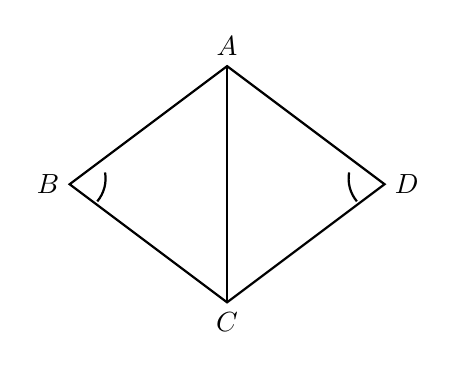
\begin{tikzpicture}[scale=1.0, thick]
  \coordinate (A) at (0,2.4);
  \coordinate (C) at (0,-0.6);
  \coordinate (B) at (-2,0.9);
  \coordinate (D) at (2,0.9);
  \draw (A) -- (B) -- (C) -- (D) -- cycle;
  \draw (A) -- (C);
  \node[above] at (A) {$A$};
  \node[left] at (B) {$B$};
  \node[right] at (D) {$D$};
  \node[below] at (C) {$C$};
  % ∠B 和 ∠D 用单弧
  \draw ($(B)+(0.45,0.15)$) arc (10:-40:0.45);
  \draw ($(D)+(-0.45,0.15)$) arc (170:220:0.45);
\end{tikzpicture}
\end{document}
